%%%%%%%%%%%%%%%%%%%%%%% file template.tex %%%%%%%%%%%%%%%%%%%%%%%%%
%
% This is a template file for Web of Conferences Journal
%
% Copy it to a new file with a new name and use it as the basis
% for your article
%
%%%%%%%%%%%%%%%%%%%%%%%%%% EDP Science %%%%%%%%%%%%%%%%%%%%%%%%%%%%
%
%%%\documentclass[option]{webofc}
%%% "twocolumn" for typesetting an article in two columns format (default one column)
%
\documentclass{webofc}
\usepackage[varg]{txfonts}   % Web of Conferences font
\usepackage{hyperref}
%\usepackage{wrapfig}
%
% Put here some packages required or/and some personnal commands
%
%
% Instructions here: https://indico.cern.ch/event/773049/page/19236-proceedings
% CHEP slides: https://docs.google.com/presentation/d/1TVrfmnRuOHwL996HmbwCpkfG34qqPawQOWzdwBy-SS4/edit#slide=id.p
% Preparation document: https://docs.google.com/document/d/1ChyrOnuZRpEdiR-A2mr4Q862CuXm9pqHMyQte6osIbM/edit#heading=h.tb97kncb2r4u


\begin{document}
%
\title{Exploiting CRIC to streamline the configuration management of GlideinWMS factories for CMS support}
%
% subtitle is optionnal
%
%%%\subtitle{Do you have a subtitle?\\ If so, write it here}

\author{\firstname{Jeffrey} \lastname{Dost}\inst{1}\fnsep\thanks{\email{jdost@ucsd.edu}} \and
        \firstname{Marco} \lastname{Mascheroni}\inst{1}\fnsep\thanks{\email{marco.mascheroni@cern.ch}} \and
        \firstname{Julia} \lastname{Andreeva}\inst{2} \and
        \firstname{Alexey} \lastname{Anisenkov}\inst{3, 4}        
        \firstname{Dennis} \lastname{Box}\inst{5} \and
        \firstname{Alessandro} \lastname{Di Girolamo}\inst{2} \and
        \firstname{Saqib} \lastname{Haleem}\inst{6} \and
        \firstname{Edita} \lastname{Kizinevi\v{c}}\inst{7} \and
        \firstname{Krista} \lastname{Majewski}\inst{5} \and
        \firstname{James} \lastname{Letts}\inst{1} \and
        \firstname{Lorena} \lastname{Lobato Pardavila}\inst{5} \and
        \firstname{Bruno} \lastname{Moreira Coimbra}\inst{5} \and
        \firstname{Antonio} \lastname{P\'{e}rez-Calero Yzquierdo}\inst{8,9} \and
        \firstname{Marco} \lastname{Mambelli}\inst{5} \and
        \firstname{Panos} \lastname{Paparrigopoulos}\inst{2} \and
        \firstname{Marian} \lastname{Zvada}\inst{10}
        % etc.
}

\institute{University of California San Diego,  La Jolla, CA, USA %9500 Gilman Dr, La Jolla, CA 92093, USA
\and
           European Organization for Nuclear Research, Meyrin, Switzerland %Espl. des Particules 1, 1211 Meyrin, Switzerland
\and
           Novosibirsk State University, Novosibirsk, Russia 
\and
           Budker Institute of Nuclear Physics, Novosibirsk, Russia
\and
           Fermi National Accelerator Laboratory, Batavia, IL, USA %Kirk Road and, Pine St, Batavia, IL 60510, USA
\and
           National Centre for Physics Rd, Islamabad, Pakistan %Islamabad Capital Territory, Pakistan
\and
           Vilnius University, Vilnius, Lithuania %Universiteto g. 3, Vilnius 01513, Lithuania
\and
           Centro de Investigaciones Energéticas Medioambientales y Tecnológicas, Madrid, Spain %Av. Complutense, 40, 28040 Madrid, Spain
\and
           Port d'Informació Científica, Barcelona, Spain %Campus UAB, Carrer de Can Magrans, s/n, 08193 Bellaterra, Barcelona, Spain
\and
           University of Nebraska-Lincoln, Lincoln, NE, USA %1400 R Street, Lincoln, NE 68588, USA
          }

\abstract{%
GlideinWMS is a workload management and provisioning system that allows sharing computing resources distributed over independent sites. Based on the requests made by GlideinWMS frontends, a dynamically sized pool of resources is created by GlideinWMS pilot factories via pilot job submission to resource sites' CEs. More than 400 CEs are currently serving more than ten virtual organizations through GlideinWMS, with CMS being the biggest user with 230 CEs. The complex configurations of the parameters defining resource requests, as submitted to those CEs, have been historically managed by manually editing a set of different XML files. New possibilities arise with CMS adopting the CRIC, an information system that collects, aggregates, stores, and exposes, among other things, computing resource data coming from various data providers. The paper will describe the challenges faced when CMS started to use CRIC to automatically generate the GlideinWMS factory configurations. The architecture of the prototype, and the ancillary tools developed to ease this transition, will be discussed. Finally, future plans and milestones will be outlined.
}
%
\maketitle
%
\section{Introduction}
\label{intro}
The Compact Muon Solenoid (CMS) experiment is one of two multipurpose experiments that collect and analyze data from proton-proton and heavy ion collisions at the Large Hadron Collider (LHC), in Geneva, Switzerland. CMS, as well as other High Energy Physics (HEP) experiments, uses Grid, Cloud, and high performance computing (HPC) centers to satisfy its computing needs, while GlideinWMS \cite{GlideinWMSSoft} is the workflow management system used by CMS to access these compute resources.

A user HTCondor \cite{HTCondorURL} pool, that shrinks and grows based on user requests, is \emph{dynamically} created by sending \emph{pilot} jobs \cite{GlideInWMS} to many resources located all around the world. Pilot jobs are responsible for validating the resources they are accessing, and then they join the user HTCondor pool in order to run user jobs. As shown in figure \ref{fig-gwms}, two components form the GlideinWMS system: a frontend and a factory.


%MM: Maybe try to wrap the figure (and the others) to save space?
%\begin{wrapfigure}{r}{0.5\textwidth}
%  \begin{center}
%    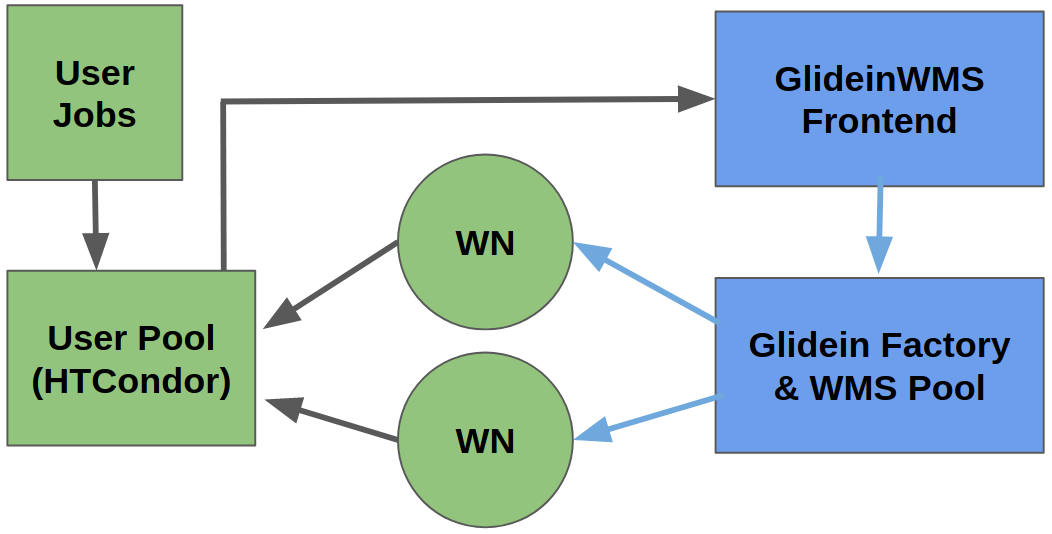
\includegraphics[width=0.4\textwidth]{images/GWMS.png}
%  \end{center}
%  \caption{The GlideinWMS system}
%\end{wrapfigure}

\begin{figure}[ht]
\centering
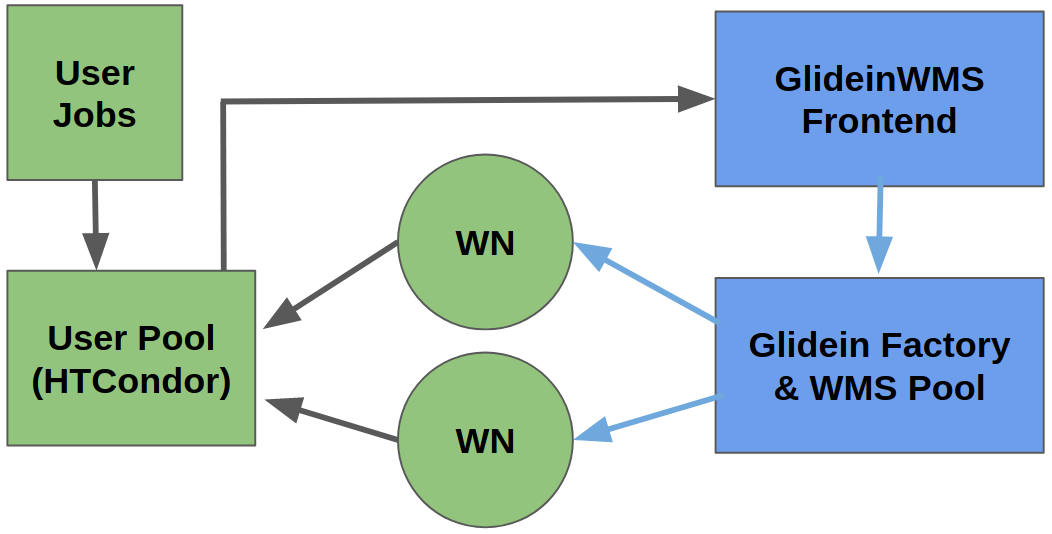
\includegraphics[width=0.5\textwidth]{images/GWMS.png}
\caption{The components of the GlideinWMS system. In order to create a dynamic HTCondor pool, a frontend and a factory work together determining the pressure from users'
jobs and sending pilot jobs to Grid, Cloud, and HPC resources. Pilot jobs running on the worker nodes then start the condor daemons that are necessary to join the central user pool, and  finally start user jobs}
\label{fig-gwms}
\end{figure}

The factory is responsible for sending the pilot jobs to the different resources. Resources belonging to the same institute form a \emph{site}. Compute Elements (CEs), the access points of Grid and HPC resources, are a set of services that provide an interface for pilot jobs to access a local resource management system, and also take care of authentication, authorization and delegation of jobs. A site can have multiple CEs, which, in turn, can have multiple \emph{queues}. Queues give the site the ability to expose different machine types, and restrict access to machines of a given type for specific user communities. In the GlideinWMS factory, \emph{entries} represent the set of parameters required to properly configure the factory to submit and run a pilot on a particular queue on a CE. The frontend looks at user and central production job pressure, and then decides how many pilot jobs the factory should send to each entry, based on the user's job requirements and the current load on each entry. Pilot jobs will first execute a set of tests to make sure the resources they are accessing are valid, checking for example that all the software necessary to execute the user jobs is installed on the worker nodes, and then they will connect to the HTCondor user pool in order to start executing user jobs. In GlideinWMS, different experiments, which are called Virtual Organizations (VOs), run one or more different frontends, which are in turn connected to one or more factories. Various multi-experiment redundant factories are used for high availability.

Factory configurations are a set of XML files that contain all of the parameters for each entry. Currently, there are more than 400 entries in those XML files which are manually maintained and correspond to about 16000 lines of XML. In this paper we discuss a new solution that CMS adopted in order to reduce the operational effort needed to maintain the factory configurations. This solution exploits the CMS Computing Resource Information Catalogue (CRIC) \cite{CRIC2017} to automatically generate a subset of the CMS factory configurations.

The rest of this paper is organized as follows. Section \ref{facops} explains more in detail how factory operations works. Section \ref{cric} introduces CRIC, while Section \ref{arch} discusses how CRIC has been used to build a prototype that can automatically generate factory configurations. Section \ref{proof} gives more detail about how the prototype has been used. Sections \ref{future} and \ref{conclusions} outline future directions and draw some conclusions, respectively.


\section{CMS Factory Operations}
\label{facops}
Factories are operated by a dedicated team of 2.5 full-time equivalent workers. The team is responsible for ensuring that the GlideinWMS system is optimally delivering useful resources to users when these are requested, while trying to minimize the waste of resources in doing so.

One of the major time-consuming activities for the factory operations team is maintaining all of the XML files containing the entries. Those configuration files have been populated over several years with site resources. %The flow chart for adding a resource is shown in figure \ref{fig-flowpre}. 
A site administrator who wants to connect their cluster to the factory and start receiving jobs from CMS opens a ticket with all of the CE queue information. Factory operators check if the information is complete and request clarifications if needed. VO-specific information is also added to the entry, and factory operators may require input from other CMS experts in order to set them. When the information is complete, the operators add the entry to a test factory. Test pilots are then sent to the site to verify all the validation scripts are executed correctly. If everything is correct, the entry can finally be added to the production factories.

The entire process of configuring, testing, and validating a new factory entry or a change to an existing entry is very time consuming and requires many interactions between the factory operations team and site administrators. It usually takes one week from the opening of the ticket to the addition of the entry to the production factory. Since plenty of room for optimization is available, the factory operations team started to evaluate possibilities to automate parts of this process.

The entire factory configuration was analyzed, and we determined there are four different categories of entry parameters:
\begin{enumerate}
\item Resource description parameters that are published in Grid-infrastructure owned information systems: CE hostname, CE type (ARC, CREAM, HTCondor, etc.), queue name, resource name, supported VOs, etc.
\item Unpublished resource description parameters: working directory, maximum number of jobs, operating system, etc.
\item Internal GlideinWMS parameters: Grid submission rates, entry names, etc.
\item VO configuration parameters: pilot CPU / memory configuration, etc.
\end{enumerate}

%\begin{figure}[ht]
%\centering
%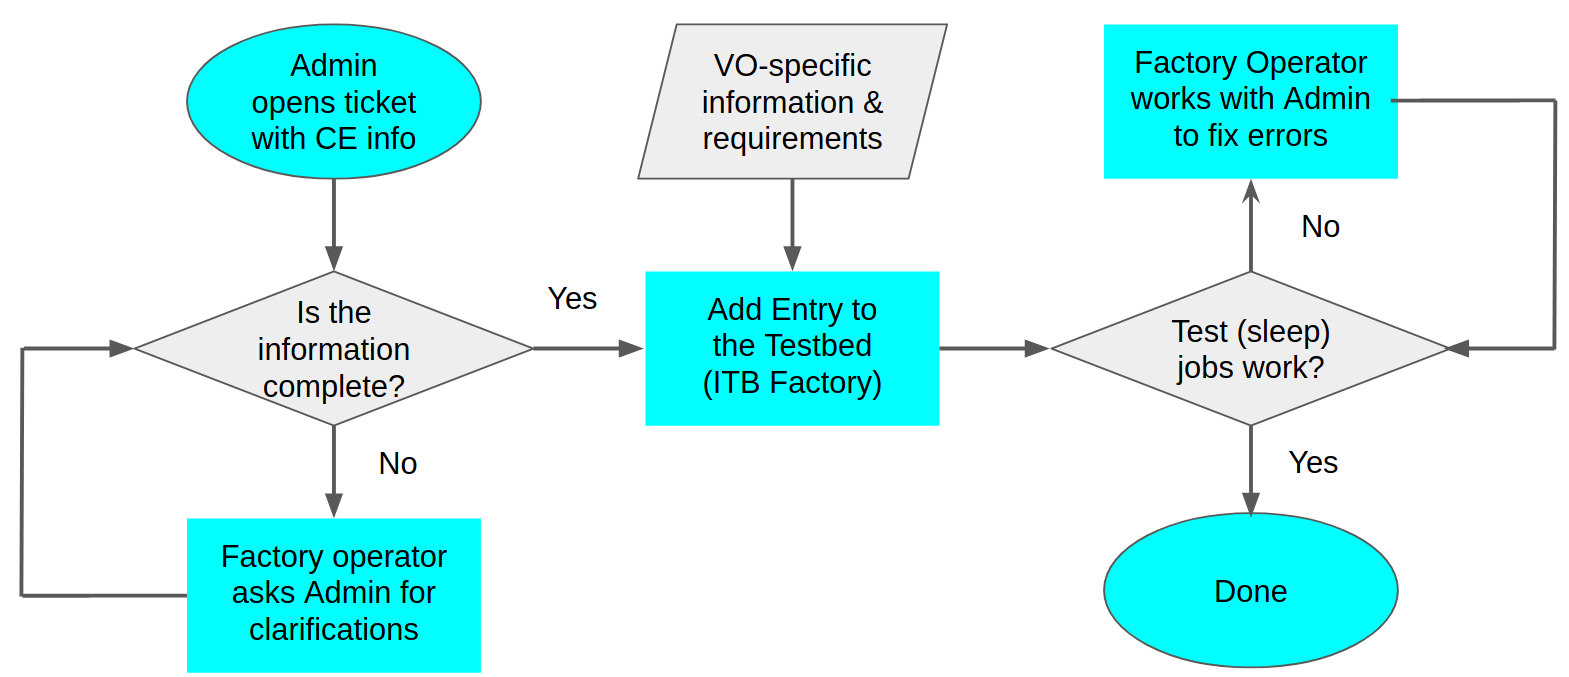
\includegraphics[width=0.8\textwidth]{images/FLOW-pre.png}
%\caption{The process of adding an entry}
%\label{fig-flowpre}
%\end{figure}

Category 1 includes attributes needed in order to submit to a given CE queue at a site. They can be found in various information systems (e.g. Open Science Grid (OSG) Topology \cite{OSG-Topology}, EGI Grid Configuration Database (GOCDB) \cite{GOCDB}), with each information system containing information about a specific set of attributes. A given site can have multiple CEs, each accessible by a physical machine hostname. There are a few implementations of CE software. In order to submit to a given CE, one must know the hostname, the implementation type and the corresponding port, and various fields may need to be set to select a queue depending on site configuration. As mentioned in Section \ref{intro}, a particular CE can expose various resource types described by queues. A queue may represent a subset of machines a VO is allowed to run on, and enforce constraints on a VO pilot that lands on the machine, such as maximum allowed memory, walltime, and number of CPUs. Depending on the CE implementation, the submission parameters might require only a logical queue name, or one may need to configure the constraints directly.

Unfortunately, the parameters available on each information systems differ and some parameters are never published, so there are parameters that 
currently a site administrator must
communicate directly to factory operators to completely configure an entry. These parameters fall under Category 2. Category 3 contains parameters that are internal to GlideinWMS, which need to be set according to factory operations experience, for example in order to regulate the pilot submission thresholds and rates by the factory for the specific resource represented in the entry. Finally, Category 4 parameters in an entry are used to configure the pilot based on VO policy. For example, a targeted resource might have up to thirty-two core machines, but CMS would prefer to configure eight core pilots to run at that site.

As discussed in Section \ref{cric}, some of the information in these categories were already available in CRIC.

\section{The Computing Resource Information Catalogue (CRIC)}
\label{cric}
In 2015 the OSG \cite{OSG} announced plans to stop using BDII \cite{BDII2010} to publish their computing resources. This triggered a review of information systems in Worldwide LHC Computing Grid (WLCG). As part of a trend in CMS (and HEP at large) to leverage community software projects, CMS began to evaluate the adoption of CRIC in 2016 as its information service. CRIC is a community project based on a refactorization of AGIS \cite{Anisenkov2017}, the ATLAS Grid Information System. %Other community projects adopted in CMS include GlideinWMS and HTCondor themselves, Rucio, and MonIT.

CRIC gathers and allows access to information about physical and logical computing resources in CMS. CRIC is made up of two components, CRIC Core, and CRIC CMS. CRIC Core provides descriptions of resources (Category 1) and gathering information from GOCDB for EGI sites, and OSG Topology for OSG sites, respectively. CRIC CMS contains experiment-specific information on how CMS organizes these resources (Category 4). For example, CRIC CMS contains the list of CMS sites available on the Grid. APIs are available to retrieve this information from both CRIC Core and CRIC CMS in JSON format.
% Circular problem
%Factory configurations used to be a data source for CRIC and were available in CRIC CMS.
In 2018, it was decided to create interfaces for factory operators in order to leverage CRIC and automate the factory configuration generation.

% MM This paragraph can be moved to a later section if needed
There are multiple advantages in this approach. CRIC represents a central and public place where all the site configurations are available via the web for everybody. The factory operations workflow can be streamlined, since less back and forth with site administrators is required to update and validate information, which in turn reduces the workload on the factory operations team. Web forms are easier to fill in than big XML files; therefore, a site administrator might be able to insert information directly into CRIC instead of factory operators doing it on their behalf. CRIC can also be used as a starting point for implementing more automated tools, such as a method to automatically send test jobs once an entry is created in CRIC.

\section{Architecture}
\label{arch}

\subsection{CRIC CMS User Interface}
\label{arch-cricui}

While CRIC Core provides a mostly complete list of all available CEs and queues per CE for a site, currently it does not provide all the details necessary to completely configure a GlideinWMS entry. In order to remedy this, the CRIC CMS component was used to bridge the missing information. In the initial integration of GlideinWMS factories with CRIC, i.e. using factories as a data source, the CMS API contains the rest of the fields necessary to complete a factory entry. CMS uses this information for other functions outside the scope of this paper, such as the SiteDB \cite{SiteDB}. In order to invert the logic so that factory entries can be generated from CRIC and at the same time not disrupt consumers of CRIC data when the factories are removed as a data source, the CRIC developers worked with factory operations to create a web-based site administrator User Interface (UI). This UI allows a site administrator or a factory operator to directly configure any fields required beyond what is already exposed in the CRIC Core API in order to complete the missing data needed to generate an entry (Categories 2-4). The site administrator UI then acts as the new input for the CMS API, which ultimately replaces the factory itself as a CRIC data source.

\subsection{Auto Entry Generation}
\label{arch-autoentry}

Two Python scripts have been deployed to run on the factory to maintain submit point entries. The first script 
%\verb"generate.py"
periodically parses the data from the CRIC JSON files and keeps an up-to-date local copy of the data on disk. The second script
%\verb"merge.py"
is responsible for merging the CRIC data with operator-provided user data, which gives the operator the ability to whitelist the desired entries to be propagated to the final factory configuration, as well as the opportunity to define new attributes, or override any attribute associated with the entry that was already retrieved from CRIC.

YAML was chosen as the file format for the intermediate files stored on disk. The reason for this is it needs to be a human-friendly readable format since operators need to look at the auto-generated files and make decisions about what to override. Factory operations experience has proven working with XML files to be cumbersome as a configuration file format that humans read and modify.

The ability to whitelist entries and manually add or override attributes are important because the factory operations team usually will perform an audit of the entry configuration and need a quick turnaround in case the generated entry is incorrect. In fact, auto-generated entries might contain errors because the data contained in Grid information not being always accurate, and fixing the errors might require long iterations with the responsible of the resource. Moreover, as discussed in Section \ref{facops}, information systems typically only contain resource attributes from Category 1, but frequently operators must fill in custom fields to properly configure the pilot for a special resource.


\section{Proof of Concept}
\label{proof}

The eight CMS Tier 2 sites in the US (UCSD, Purdue, Caltech, Florida, MIT, Nebraska, Wisconsin, and Vanderbilt) were selected as candidates to test the auto-generation of entries from CRIC data. YAML whitelist files were manually edited, and the new scripts were used to automatically generate the factory XML configuration in a production environment. These sites were ideal because they are representative of most of the entries in the factory configuration. Figure~\ref{fig-baconf} illustrates the immediate gains due to integrating the improved setup. Before having the ability to auto-generate the entries, most of the configuration that would have been put in place by hand would have contained lots of repetitive template code that is prone to error. This boiler plate code is now pulled from the default YAML file instead. Resource-specific fields are almost completely taken from a combination of CRIC Core and site administrator UI. The manual override YAML file that the factory operator must maintain is reduced to simply whitelisting the entry, and overriding a handful of fields as needed. Besides the great simplification of the configuration file, there is a reduction in the number of interactions between site administrator and factory operator, since the site administrator has direct control of the fields describing their site by virtue of the CRIC UI, and consequently a reduction in time needed to deploy an entry.

\begin{figure}[ht]
\centering
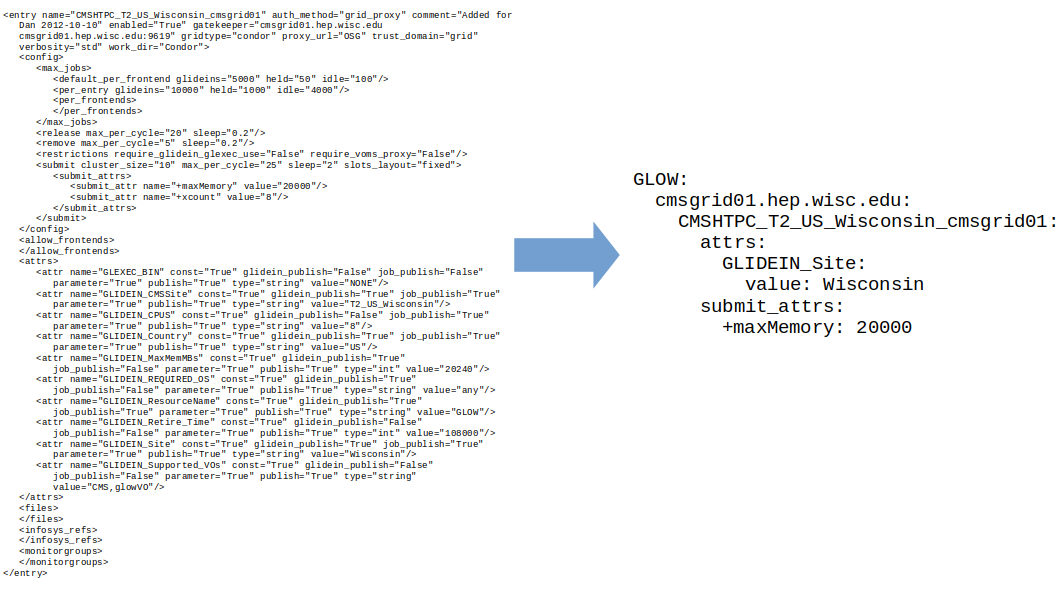
\includegraphics[width=1.0\textwidth]{images/before_after_conf.png}
\caption{Old manual XML entry compared to the new YAML override entry. The reduction in the number of lines to maintain is clearly visible since most of the XML parameters are now in CRIC or the default YAML file}
\label{fig-baconf}
\end{figure}

While running the auto-generation in a production environment has proven successful, there is still some room for improvement in the current implementation. The first issue is that the site administrator UI is still predominantly designed from the perspective of factory operations team. For example, the list of accepted VO has specific naming schemes that are case-sensitive and are internal to factory operations. A site administrator would not know to put "CMS instead of "cms", "OSGVO" instead of "osg", and so on. Similar conventions exist for Operating System (OS) flavor. For example, knowing to spell out "RHEL7" instead of "sl7", and worse, knowing to use the special key word "any" if the site supports containers. Finally, a site administrator would have to know that factory operations uses specific units for numeric fields, like seconds for maximum walltime, or megabytes for maximum memory. These are only a few examples of why configuring a factory entry is not very user-friendly for a site administrator.

Another limitation of the current implementation is that initially the factory operations team focused only on the auto-generation of CMS entries. However, the scope of factory operations is beyond CMS and WLCG. 
%It would not be appropriate to have non-WLCG site administrators use CRIC to configure entries. 
For example, there are some exotic configurations specific to non-CMS VOs that do not need to be considered in the CMS CRIC case and would only over-complicate the implementation. The longer term solution for auto-generation of entries for factory operations as a whole should work for all sites. CRIC gives factory operations the extra help in auto-generating CMS and WLCG entries, but other tools will need to be developed to interface other external information systems and databases to handle the non-WLCG, non-CMS sites that the factory also supports.

%MM I would add here at the end of the proof of concept the chart with the improved workflow as well

%\begin{figure}[ht]
%\centering
%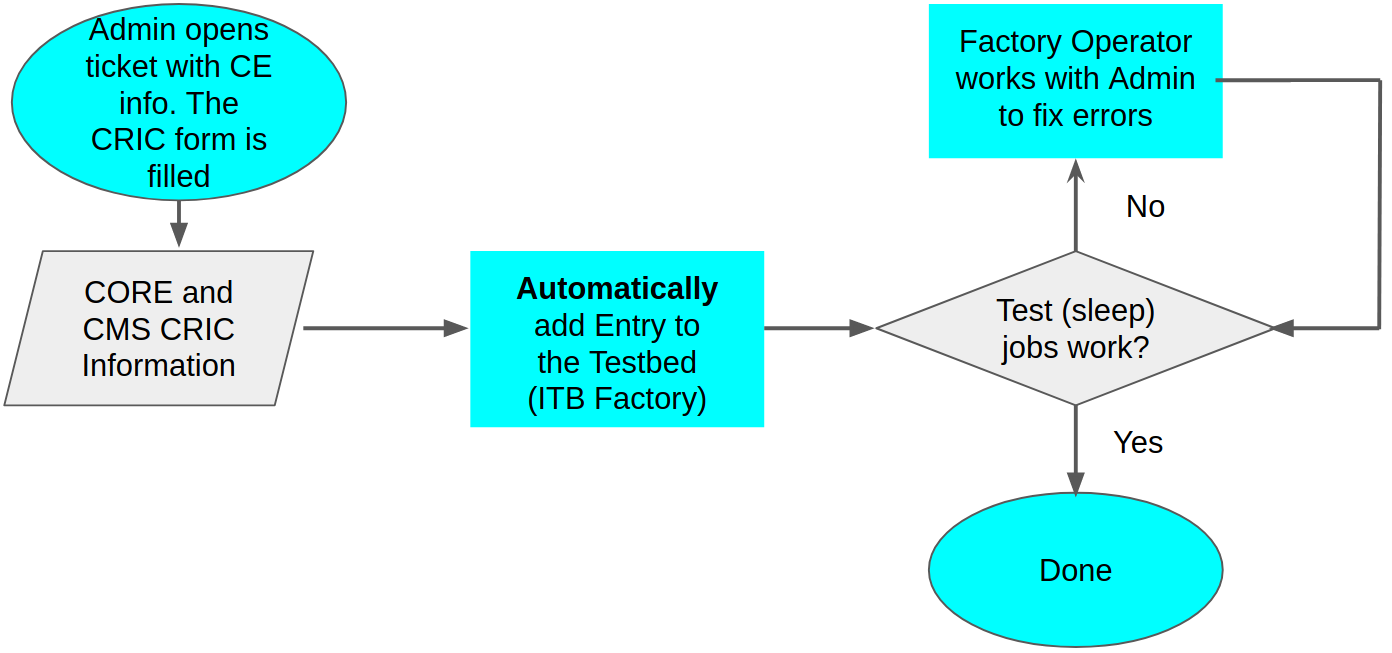
\includegraphics[width=0.8\textwidth]{images/FLOW-post.png}
%\caption{Improved process of adding an entry}
%\label{fig-flowpost}
%\end{figure}

\section{Future Plans}
\label{future}
% describe improvements we are working on

In order to address the issues discussed in Section ~\ref{proof}, we have begun developing a new implementation focusing on OSG CEs that are not in CRIC. The OSG CE Collector is the OSG replacement of BDII. It is a simple HTCondor collector that contains descriptions of all of the CEs in the OSG. Coincidentally, it is one of the data sources CRIC Core consumes for WLCG sites in the OSG. The idea behind the new implementation is to use CRIC for all sites where it is appropriate, then for non-WLCG OSG sites, directly parse the OSG CE Collector for the data required to configure the entries. One downside is for these sites, site administrators do not get the nice CRIC UI. However for OSG it is not an issue because administrators are used to using the OSG Configure tools to propagate the resource descriptions into the OSG CE Collector. Learning how OSG Configure works has also given the factory operations team a better understanding what a site administrator-centric interface looks like. So the operations team can take this and work with the CRIC developers to decouple the factory specific peculiarities of the current entry creation interface, and improve the user experience for site administrators.

\section{Conclusions}
\label{conclusions}
The CMS GlideinWMS factory is an important piece of the computing infrastructure of CMS. It has been historically operated by managing a set of XML files which contains more than 400 entries, corresponding to about 16000 lines of XML. In order to reduce the effort needed to maintain the factory, the factory and the CRIC teams worked together on a new solution that allows CMS factory operators to leverage the CRIC interface to insert and manage entries. 

The solution has been validated in a production environment, and the factory operations team is now evaluating how to address a wider variety of use cases in addition to CMS VO and WLCG Sites.

\section*{}
\label{acknowledgements}

\begin{acknowledgement}
This work was partially supported by the U.S. Department of Energy, the National Science Foundation, and by Spain’s Ministry of Economy and Competitiveness grant FPA2016-80994. CMS thanks our partners in the GlideinWMS, HTCondor, and CRIC development teams, the OSG, and our colleagues at CERN, all of whom make the shared computing infrastructure a success.
\end{acknowledgement}

%For bibliography use \cite{RefJ}

% BibTeX or Biber users please use (the style is already called in the class, ensure that the "woc.bst" style is in your local directory)
\bibliography{papers}
%
% Non-BibTeX users please use
%
%\begin{thebibliography}{}
%
% and use \bibitem to create references.
%
%\bibitem{RefJ}
% Format for Journal Reference
%Journal Author, Journal \textbf{Volume}, page numbers (year)
% Format for books
%\bibitem{RefB}
%Book Author, \textit{Book title} (Publisher, place, year) page numbers
% etc
%\end{thebibliography}

\end{document}